% !TeX spellcheck = en_GB
% /*
%  * ----------------------------------------------------------------------------
%  * "THE BEER-WARE LICENSE" (Revision 42):
%  * Fabian Hauser wrote this file. As long as you retain this notice you
%  * can do whatever you want with this stuff. If we meet some day, and you think
%  * this stuff is worth it, you can buy me a beer in return. Fabian Hauser
%  * ----------------------------------------------------------------------------
%  */

\documentclass[
a4paper,
oneside,
10pt,
fleqn,
headsepline,
toc=listofnumbered, 
bibliography=totocnumbered]{scrartcl}

% deutsche Trennmuster etc.
\usepackage[T1]{fontenc}
\usepackage[utf8]{inputenc}
\usepackage[english, ngerman]{babel} % \selectlanguage{english} if  needed
\usepackage{lmodern} % use modern latin fonts

% Custom commands
\newcommand{\AUTHOR}{Fabian Hauser \& Muriele Trentini}
\newcommand{\INSTITUTE}{Hochschule für Technik Rapperswil}
\newcommand{\GITHUB}{https://github.com/michiwieland/hsr-zusammenfassungen}
\newcommand{\LICENSEURL}{https://en.wikipedia.org/wiki/Beerware}
\newcommand{\LICENSE}{
"THE BEER-WARE LICENSE" (Revision 42):
<michi.wieland@hotmail.com> wrote this file. As long as you retain this notice you
can do whatever you want with this stuff. If we meet some day, and you think
this stuff is worth it, you can buy me a beer in return. Michael Wieland	
}

% Jede Überschrift 1 auf neuer Seite
\let\stdsection\section
\renewcommand\section{\clearpage\stdsection}

% Multiple Authors
\usepackage{authblk}

% Layout / Seitenränder
\usepackage{geometry}

% Inhaltsverzeichnis
\usepackage{makeidx} 
\makeindex

\usepackage{url}
\usepackage[pdfborder={0 0 0}]{hyperref}
\usepackage[all]{hypcap}
\usepackage{hyperxmp} % for license metadata

% Glossar und Abkürzungsverzeichnis
\usepackage[acronym,toc,nopostdot]{glossaries}
\glossarystyle{altlisthypergroup}
\usepackage{xparse}
\DeclareDocumentCommand{\newdualentry}{ O{} O{} m m m m } {
	\newglossaryentry{gls-#3}{name={#5},text={#5\glsadd{#3}},
		description={#6},#1
	}
	\makeglossaries
	\newacronym[see={[Siehe:]{gls-#3}},#2]{#3}{#4}{#5\glsadd{gls-#3}}
}
\makeglossaries

% Mathematik
\usepackage{amsmath}
\usepackage{amssymb}
\usepackage{amsfonts}
\usepackage{enumitem}

% Images
\usepackage{graphicx}
\graphicspath{{images/}} % default paths

% Boxes
\usepackage{fancybox}

%Tables
\usepackage{tabu}
\usepackage{booktabs} % toprule, midrule, bottomrule
\usepackage{array} % for matrix tables

% Multi Columns
\usepackage{multicol}

% Header and footer
\usepackage{scrlayer-scrpage}
\setkomafont{pagehead}{\normalfont}
\setkomafont{pagefoot}{\normalfont}
\automark*{section}
\clearpairofpagestyles
\ihead{\headmark}
\ohead{\AUTHOR}
\cfoot{\pagemark}

% Pseudocode
\usepackage{algorithm}
\usepackage{algorithmic}

% Code Listings
\usepackage{listings}
\usepackage{color}
\usepackage{beramono}

\definecolor{DarkPurple}{rgb}{0.4, 0.1, 0.4}
\definecolor{DarkCyan}{rgb}{0.0, 0.5, 0.4}
\definecolor{LightLime}{rgb}{0.3, 0.5, 0.4}
\definecolor{Blue}{rgb}{0.0, 0.0, 1.0}

\lstdefinestyle{eclipse-style}{
	language=Java,  
	columns=flexible,
	showstringspaces=false,     
	basicstyle=\footnotesize\ttfamily, 
	keywordstyle=\bfseries\color{DarkPurple},
	commentstyle=\color{LightLime},
	stringstyle=\color{Blue}, 
	escapeinside={£}{£}, % latex scope within code      
	morekeywords={length},
	numbers=left,
	numberstyle=\tiny\color{black},
	frame=single,
}
\lstset{style=eclipse-style}


% Theorems \begin{mytheo}{title}{label}
\usepackage{tcolorbox}
\tcbuselibrary{theorems}
\newtcbtheorem[number within=section]{definiton}{Definition}%
{fonttitle=\bfseries}{def}
\newtcbtheorem[number within=section]{remember}{Merke}%
{fonttitle=\bfseries}{rem}

% Template extensions
\newcommand\equalhat{\widehat{=}}
\newcommand\mathSpaceSeparator{\text{ }\text{ }\text{ }\text{ }}


% Dokumentinformationen
\newcommand{\SUBJECT}{Zusammenfassung}
\newcommand{\TITLE}{Programmieren und Formale Methoden}
\def\tabmath\[#1\]{\vspace{2ex}$\displaystyle#1$}

\loadglsentries{glossar}

% pdf metadata
\hypersetup{
	pdfauthor={\AUTHOR},
	pdftitle={\SUBJECT \TITLE},
	pdfcopyright={\LICENSE},
	pdflicenseurl={\LICENSEURL}
}

\begin{document}
	
% Front page
\title{\TITLE}
\subject{\SUBJECT}
\author{\AUTHOR}
\affil{\INSTITUTE}
\date{\today}
\maketitle

\vfill

% Participate
\paragraph{Mitmachen} \hfill \\
Falls Du an diesem Dokument mitarbeiten willst, kannst Du das Dokument
auf GitHub unter \url{\GITHUB} forken.

% Licence
\paragraph{Lizenz} \hfill \\
\LICENSE

% Table of contents
\tableofcontents


% Glossar and acronyms (if included \loadglsentries{glossar})
\printglossary[type=\acronymtype]
\printglossary
\glsaddall


\section{Introduction}
The use of a formal language to describe and solve problems is central to computer science.

\begin{description}
	\item[Formal Methods] the application of theoretical computer science fundamentals. Motivation: use of mathematical analysis make computer programming more reliable and predictable.
	\item[Formal Language] Set of strings of symbols that are constrained by specific rules. Membership in this set can automatically be determined (mechanical processing possible)
	\item[Informal Language] Any living natural language
\end{description}

\section{Programming Paradigms}

Paradigm is a Worldview / Concept / Tought patterns.

OOP uses multiple of the paradigms below, but is not a paradigm in this sense.

\subsection{The Imperative Programming Paradigm}

Is imperative (de: Befehlend) and focuses on \emph{how} a program works, like a recipe. It uses commands to change the program's state.

A program (in this course) is a sequence of commands and the computation is a change of state.

Most hardware implementations of computer is imperative.

It is based on the Von Neumann architecture.

\subsubsection{Basic Building Blocks}

\begin{description}
	\item[Assignments (sate/store/heap)] \lstinline|x:= x+1|
	\item[Sequential composition] \lstinline|...; ...|
	\item[Conditional exception] \lstinline|if ... then ... else...|
	\item[Repetition] \lstinline|while .. do .. / goto ...|
\end{description}



\subsection{The Declarative Programming Paradigm}

Describe logic of computation without explicitly describing its control flow.

\emph{What} should a program accomplish, not how the language should do something (But it must still be computable in the end).

Programs are here theories of a formal logic. Computations are deductions.

Examples: Spreadsheets, Regex, Query Languages (SQL etc.), Functional programming languages (Haskel, ...), Logic programming (Prolog)

\subsubsection{The Functional Programming Paradigm}

Basis: The Lambda Calculus

Programs are function definitions, computations are function evaluations.

\subsubsection{The Logical Programming Paradigm}
Basis: Predicate logic

Programs are rules in predicate logic and computation is a proof of a predicate.



\section{Formal Proof (Propositional and Predicate logic)}

\begin{figure}
	\centering
	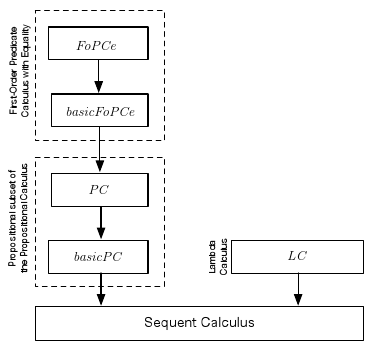
\includegraphics[width=0.7\linewidth]{images/sequent_calculus_overview}
	\caption{Overview calculus proof family.}
	\label{fig:sequentcalculusoverview}
\end{figure}

\subsection{refresher ''Diskrete Mathematik''}
Kinds of logic: Boolean, ''Aussagenlogik'' ($\neg, \wedge, \vee,  \Rightarrow, \Leftrightarrow$), ''Prädikatenlogik'' ($\forall,\exists, R(x)$)

Proofs: by induction, direct, indirect, by contradiction

\subsection{What are formal and informal proofs?}
In an \emph{informal proof} arguments are presented as explanations in natural language (like most mathematical textbooks; needs a human to check correctness)

A \emph{formal proof} is constructed using well-formed formulas of a formal language and formally defined rules of inference.
 They can be checked by a machine and sometimes be mechanically constructed. Computer programs are able to assist proving (e.g. like Excel), sometimes a proof is even not practically possible without them.

\subsection{Sequent Calculus style}

The sequent calculus style is widely used in computer science, for instance to define program semantics or typing rules.

\subsection{Sequent Calculus}
A sequent is a generic name for a statement that we want to prove.
\subsubsection{Proof Rules}

A device to construct proofs.

\[
\frac{\overrightarrow{A}}{C} \boldsymbol{r}
\]

\begin{description}
	\item[$r$] Rule name
	\item[$C$] Consequent (to be proven)
	\item[$\vec{A}$] Antecedents: list of sequents (vector).
\end{description}


We want to proof $C$ out of multiple sequent proof rules $A_1, A_2, ..., A_n$ with the rule $r$. If there is no $A$ above the line, the proof rule is an axiom. The order of proof rules in $A$ is important and not permutable.

To build a complete proof, all proof rules must be proven up to an axiom.


\subsubsection{Definitions}

\begin{description}
	\item[Sequent] a generic name for a statement that
we want to prove.
	\item[Proof Rule] A rule $r$ to proof a consequent $C$ with sequents in $A$
	\item[pending sub-goal] A sequent which is not yet proven by an axiom.
	\item[Axiom] Proof rule without sequent $A$; basic element assumed to be true. \\
	There should be as few axioms as possible.
	\item[Calculus (or Theory)] (possibly infinite) set of proof rules $r_1$, $r_2$.
	\item[Proof (or Derivations)] Ordered proof rules in a tree, so that all proof rules are proven by an axiom.
	\item[incomplete Proof] has at least one pending subgoal
\end{description}

\subsubsection{Example}

\paragraph{Type checking proof}

of the shorthand if else construct for integers.

\[
	\frac{
			\frac{
				\frac{}{x::int}x_{int} \text{   } \frac{}{y::int}y_{int}
			}{(x > y)::bool}>_{int} \text{   }
		  \frac{
				\frac{}{x::int}x_{int} \text{   } \frac{}{y::int}y_{int}
			}{(x - y)::int} -_{int1} \text{   }
			\frac{
				\frac{}{y::int}y_{int} \text{   } \frac{}{x::int}x_{int}
			}{(y - x)::int} -_{int2}
		}{(x>y? x - y : y - x)::int} condExpr_{int}
\]

\subsection{Propositional Calculus (DE: Aussagenlogik)}

Example:\\*
If it is raining then it is cloudy.\\*
It is raining.\\*
Therefore it is cloudy.

\subsubsection{Definitions}
\begin{description}
	\item[Predicate] Truth value that we can assume or wish to prove (also called proposition).
	\item[Sequent] $H \vdash G$, read: Under the hypotheses $H$, prove the goal $G$ \hfill \\
	\begin{description}
		\item[$H$] Hypoteheses: a (finite) set of predicates
		\item[$\vdash$] therefore/entails
		\item[$G$] Goal: a single predicate
	\end{description}
\end{description}

\subsubsection{basicPC: Basic Propositional Calculus}

The basicPC syntax is the minimal subset required to write propositional logic. The syntax is defined in BNF (Bacus-Naur-Form).

\[
	P ::= \bot | \neg P | P \land P | P
\]

The rules above are a logical \emph{NAND}, which are also the most basic element of electronical circuits.

\subsubsection{Proof Rule Schema}

Proof Rule schemas represent an infinite number of proof rules of the same form. They use ''meta variables'', that can be instantiated (that is, replaced).

\paragraph{Example} 
\[
	\frac{
		\text{H} \vdash P \mathSpaceSeparator \text{H}, P \vdash C
	 }{
		\text{H} \vdash Q
	} cut
\]

In this example, H, $P$ and $Q$ are meta-variables that need to be initiated with concrete predicates, e.g. $A$, $B$ and $C$: \begin{align*}
  \text{H} &:= \{A\} \\
	P &:= B \\
	Q &:= C \\
\end{align*}

Commas, like in the example $\text{H}, P \vdash C$, are used to create a new set containing alle elements from H and $P$.

\subsubsection{Proof Rules of basicPC}
\begin{table}[h]
	\centering
	\begin{tabu} to \linewidth {l X}
		\toprule
		Formula & Description \\
		\midrule
		\tabmath\[\frac{}{\text{H},P \vdash P} hyp \] &
			If P is in hypothesis and goal the sequent is proven \\
		\tabmath\[ \frac{\text{H} \vdash Q}{\text{H},P \vdash Q} mon \] &
			We can leave out individual Hypotheses \\
		\tabmath\[ \frac{\text{H} \vdash P \mathSpaceSeparator \text{H}, P \vdash Q}{\text{H} \vdash Q} cut \] &
			Allows you to introduce lemmas to simplify proving  $H \vdash Q$ \\
		\tabmath\[ \frac{}{\text{H}, \bot \vdash P} \bot hyp \] &
			With an inconsistent system, you are able to prove anything. \\
		\tabmath\[ \frac{\text{H}, \neg P \vdash \bot}{\text{H} \vdash P} contr \] &
			Proof by contradiction: If we assume P is false, our hypotheses are inconsistent. \\
		\tabmath\[ \frac{\text{H}, P \vdash \bot}{\text{H} \vdash \neg P} \neg goal \] &
			negations can ''jump'' over turnstile \\
		\tabmath\[ \frac{\text{H} \vdash P}{\text{H}, \neg P \vdash Q} \neg hyp \] &
			negations can ''jump'' over turnstile \\
		\tabmath\[ \frac{\text{H} \vdash P \mathSpaceSeparator \text{H} \vdash Q}{\text{H} \vdash P \land Q} \land goal \] &
			If we want to prove $P \land Q$ , we can prove $P$ and $Q$ separately. \\
		\tabmath\[ \frac{\text{H},P,Q \vdash R}{\text{H},P \land Q \vdash R} \land hyp \] &
			If we have a conjunction in Hypothesis, we can assume the Hypotheses separately \\
		\bottomrule
	\end{tabu}
	\label{tbl:ProofRulesBasicPC}
	\caption{Proof Rules of basicPC}
\end{table}


\subsubsection{Operators}

The $\equalhat$-Sign denotes a syntactic equivalence.

\begin{align*}
	\top & \equalhat \neg \bot 
	& \text{( $\equalhat_{\top}$)} \\
	P \lor Q & \equalhat \neg(\neg P \land \neg Q)
	& \text{( $\equalhat_{\lor}$)} \\
	P \Rightarrow Q & \equalhat \neg P \lor Q
	& \text{( $\equalhat_{\Rightarrow}$)} \\
	P \Leftrightarrow Q & \equalhat (P\Rightarrow Q) \land (Q \Rightarrow R)
	& \text{( $\equalhat_{\Leftrightarrow}$)} \\
\end{align*}

\emph{Important}: Both proof rules and syntactic rewriting can be used in a single proof!

\subsubsection{Additional Proof Rules}

There are additional proof rules, that are based on the newly introduced logical operators can now be derived:

\begin{figure}[h]
\centering
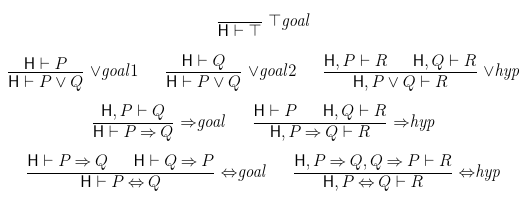
\includegraphics[width=0.7\linewidth]{images/pc_additional_proof_rules}
\caption{Additional Proof Rules of PC}
\label{fig:pcadditionalproofrules}
\end{figure}



\subsection{First order Predicate Calculus}

We would like to extend predicate calculus PC to FoPCe via an intermediate step basicFoPCe to also allow Mathematical objects (numbers, functions, things, people etc.)

\subsubsection{Definition}

\begin{description}
	\item[FoPCe] first-order predicate calculus with equality
	\item[Expression] An expression is a formal statement denoting a mathematical object. Expressions cannot be proven. Examples: $f(x), x, g(x, f(x))$
	\item[Variables] A variable is an identifier that denotes an expression. It is just a place holder and may be a black box. Example: $x$
\end{description}

\subsubsection{Syntax}
\begin{align*}
	P &::= ...| \forall x.P | E = E | R(\vec{E}) 
	& \text{where R() and “=” are uninterpreted/special relationship symbols}\\
	E &::= x | f(\vec{E})
	& \text{where $\vec{E}$ is a List of Expressions}
\end{align*}	

\paragraph{Free and bound variables} \[
	\forall x .(f(x,y) = a \land A)
\]

$x$ is a bound variable: it is just a place holder. It's name has no significance and can be changed.

$y$ is a free variable that can be assigned ''externally''.

\subsubsection{Proof rules for basicFoPCe}
\begin{figure}[H]
\centering
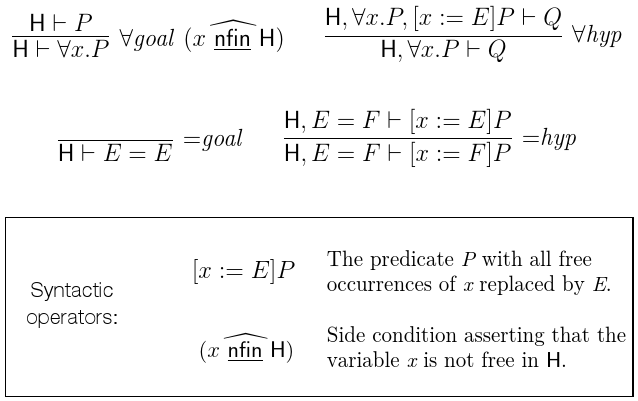
\includegraphics[width=0.7\linewidth]{images/basicfopce_proof_rules}
\caption{Proof rules of basicFoPCe}
\label{fig:basicfopceproofrules}
\end{figure}

\subsubsection{Excursion: Computation using FoPCe}
Example: We want to compute the reachability of nodes in a graph

\begin{figure}[H]
\centering
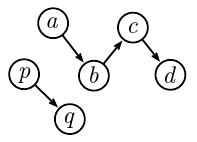
\includegraphics[width=0.2\linewidth]{images/fopce_graph_excursion}
\caption{Excursion: Computation using FoPCe Graph}
\label{fig:fopcegraphexcursion}
\end{figure}

Step 1: Model the problem as a sequent in FoPCe \\

Nodes in a graph have a relationship \\
$R(x,y)$\qquad Denotes that node y can be reached from node x\\

We need a set of Hypotheses 'G' \\
Reflexive: $\forall x. R(x,x)$ \\
Transitiv: $\forall x.\forall y.\forall z. R(x,y) \land R(y,z) \Rightarrow R(x,z)$

Our specific Graph:\\
$R(a,b) \qquad R(b,c) \qquad R(c,d) \qquad R(p,q)$\\

Our Queries: \\
\begin{align*}
	&\text{Is node a reachable from node d:} &G &\vdash R(a,d)\\
	&\text{Which nodes are reachable from node a:} &G &\vdash \exists x.R(a,x)
\end{align*}

\subsubsection{Excursion: Equational Reasoning}
Equational reasoning is a different style of a formal proof \textbf{equivalent} to FoPCe Proofs. It is however specialized for proofs \emph{only involving equality}.

\begin{figure}[H]
\centering
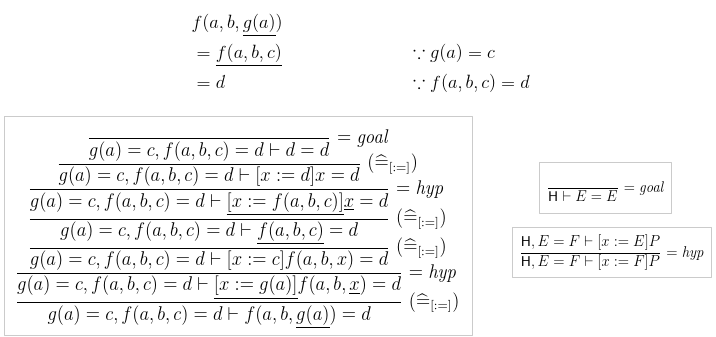
\includegraphics[width=0.8\linewidth]{images/fopce_equational_reasoning}
\caption{Excursion: Equational Reasoning with equivalent FoPCe}
\label{fig:fopceequationalreasoning}
\end{figure}

\section{Logic programming (Prolog)}
A Prolog program consists of a knowledge base (i.e. an intelligent database), which consists od rules and facts, and a query.
If you run the query, Prolog will answer with either “true” or “false”, depending on whether a proof could be found.
\subsection{First Prolog program}
We want to compute the validity of this syllogism: \\
All humans are mortal. \\
Socrates is human. \\
Therefore, Socrates is mortal.\\
Step 1: Model the argument as a sequent in FoPCe

\[
\text{H(x): x is human}\\
\text{M(x): x is mortal}\\
\text{s: Sokrates}\\
\forall x.H(x) \Rightarrow M(x),H(s) \vdash M(s)
\]

Step 2: Use Prolog to find a proof for the sequent

\begin{figure}[H]
\centering
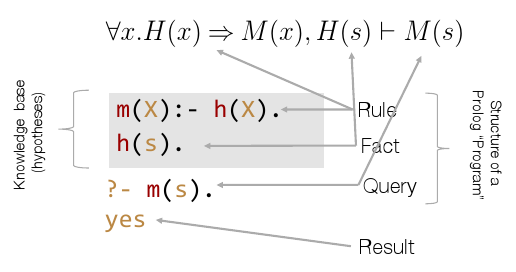
\includegraphics[width=0.6\linewidth]{images/prolog_logic_conversion}
\caption{Prolog / Logic conversion ''Hello World''}
\label{fig:prologlogicconversion}
\end{figure}

\subsection{Programming in Prolog}
Prolog requires a different mindset, as it uses:
\begin{itemize}
	\item Declarative syntax (not procedural)
	\item Recursion only (no ''for'' or ''while'' loops)
	\item Relations (no functions)
	\item Unification
\end{itemize}

\subsubsection{Fact, Rules \& Queries}

\paragraph{Knowledge Base} \hfill \\
	A collection (usually a file) of Facts.

\paragraph{Fact} \hfill \\
	Hard Facts, e.g. \lstinline|woman(mia).| or a simple fact \lstinline|party.|

\paragraph{Rules} \hfill \\
	Something is true, if something else is also true, e.g.  \lstinline|playsAirGuitar(mia):= listens2music(mia).|


Undefined predicates (e.g. \lstinline|tatooed(mia)|) can either result in \lstinline|no| or an error-message.

\paragraph{Conjunction (AND)}

is expressed by a comma.
\begin{lstlisting}[language=Prolog]
playsAirGuitar(vincent):-
  listens2music(vincent),
  happy(vincent).
\end{lstlisting}


\paragraph{Disjunction (OR)}

is expressed by a semicolon.
\begin{lstlisting}[language=Prolog]
playsAirGuitar(butch):-
listens2music(butch);
happy(butch).
\end{lstlisting}

\paragraph{Overview Logic} \hfill \\ 

\begin{table}[H]
	\centering
	\begin{tabu} to \linewidth {l l l}
		\toprule
		What & Prolog & Logic \\
		\midrule
		Implication & \lstinline|A:-B| & B $\implies$ A \\
		Conjunction & \lstinline|A,B| & A $\land$ B \\
		Disjunction & \lstinline|A;B|  & A $\lor$ B \\
		\bottomrule
	\end{tabu}
	\label{tbl:prologLogicOverview}
	\caption{Prolog Logic Overview}
\end{table}

\subsubsection{Language Components}

\paragraph{Atoms}

Atoms can have following forms: 

\begin{description}
	\item[Lowercase word] \hfill \\
		\lstinline|butch|, \lstinline|big_kahuna_burger| or \lstinline|playGuitar|
	\item[Arbitrary sequence enclosed in single quotes] \hfill \\
		\lstinline|'Vincent'|, \lstinline|'Five dollar shake'|, \lstinline|'@$%'|
	\item[Sequence of special characters] \hfill \\
		\lstinline|;..:-.|
\end{description}

\paragraph{Variables}

Are written in Uppercase, e.g. \lstinline|woman(X).| or with a beginning underscore. Prolog tries to find all Facts (in this case, names of woman) that match \lstinline|X|.

Examples: \lstinline|X|, \lstinline|Y|, \lstinline|Variable|, \lstinline|Vincent|, \lstinline|_tag|

In combination with a conjunction: \lstinline|loves(marsellus, X), woman(X).|

We can also write predicates with Variables: 
\begin{lstlisting}[language=Prolog]
jealous(X,Y):- loves(X,Z), loves(Y,Z).

?- jealous(marsellus,W).
\end{lstlisting}

\paragraph{Arity}

Number of Arguments (e.g. \lstinline|woman(X)| $\rightarrow$ arity 1)

You can define the same function with different arities. They are stored as e.g. \lstinline|woman/1| or \lstinline|jealous/2|

\paragraph{Unification}

Two terms unify, if they are \emph{exactly} the same. If you have a Variable in one Term, the instanceiation (with a concrete, equal value) is unified.

In Prolog, you can check unification with the \lstinline|=|-Symbol. E.g. \lstinline|mia = mia.| Important: the Term must be finite (or Prolog tries to output a infinite function nesting.)

Some more examples:
\begin{lstlisting}[language=Prolog]
?- X=mia, X=vincent.
no % because X cannot be mia and vincent at the same time.

?- a(f(e),X) = a(Y,k(s)).
X = k(s)
Y = f(e)
yes
\end{lstlisting}

We can enforce specific terms to to unify (even if they are infinite):
\lstinline|unify_with_occurs_check(father(X),X)|

\paragraph{Parse Tree}

Runs from the left to the right and creates according subtrees.


\subsubsection{Recursion}

A statement \lstinline|p:-p.| does logically make sense - but will result in a endless recursion executed in prolog.

\paragraph{Building a recursion} \hfill \\

To build a recursion, take following steps:

\begin{enumerate}
	\item Write down the signature of the predicate
	\item Choose parameters over which you want to perform recursion
	\item Identify and write down the case distinctions for the recursion parameters on the left hand side of the rules.
	\item The case distinctions consist of \emph{base} cases and \emph{recursive} cases.
	\item For each recursive case, note down the predicate applied to the input parameter(s) made ''smaller''. The predicate may be used within the right hand side of your rule.
	\item Complete your rules.
	\item Check that your rules are valid properties of the predicate you want to define.
\end{enumerate}

\paragraph{Example 1} \hfill \\

\begin{lstlisting}[language=Prolog]
child(anna, bridget).
child(bridget,caroline).
child(caroline,donna).
child(donna,emily).
descend(X,Y):- child(X,Y).
descend(X,Y):- child(X,Z), descendend(Z,Y).
\end{lstlisting}

\paragraph{Example 2} \hfill \\

\begin{lstlisting}[language=Prolog]
numeral(0).
numeral(succ(X)):- numeral(0).

?- numeral(succ(succ(succ(0)))).
%Yes
\end{lstlisting}

\subsubsection{Lists}

\begin{lstlisting}[language=Prolog]
?- [Head|Tail] = [a,b,c].
Head = [a]
Tail = [b,c]
\end{lstlisting}


\paragraph{member/2} \hfill \\

\begin{lstlisting}[language=Prolog]
member(X, [X|T]).
member(X,[H|T]):- member(X,T).
\end{lstlisting}

\subsubsection{Arithmetics}

With Prolog, you can do following mathematical operations: $+$, $*$, $-$, $/$, $mod(7,2)$. These are really all \lstinline|/2|-expressions. To ''assign'' results, you have to use \lstinline|is/2|.

Also, it is possible to compare integers:
\begin{figure}[h]
\centering
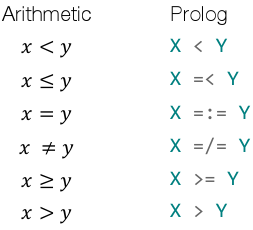
\includegraphics[width=0.2\linewidth]{images/integer_comparison}
\caption{Integer comparisons}
\label{fig:integercomparison}
\end{figure}


\begin{lstlisting}[language=Prolog]
?- X is 4+2.
X = 6
\end{lstlisting}

Can also be written as \lstinline[language=Prolog]|is(4,3+1)| or also \lstinline[language=Prolog]|is(4,+(3,1))|

\subsubsection{Accumulators (Tail Recursions)}

Tail recursion reduces the parse tree, as there are not multiple recursion possibilities. Once you reach the base clause, the result is already calculated.

\lstinline|acclen/3|

\begin{lstlisting}[language=Prolog]
acclen([], Acc, Length):- Length = Acc.

acclen([_|L], OldAcc, Length):-
NewAcc is OldAcc + 1,
acclen(L, NewAcc, Length).

length(List, Length):- acclen(List, 0, Length).
\end{lstlisting}

\paragraph{Parse Tree comparision} \hfill \\

\begin{figure}[h]
	\centering
	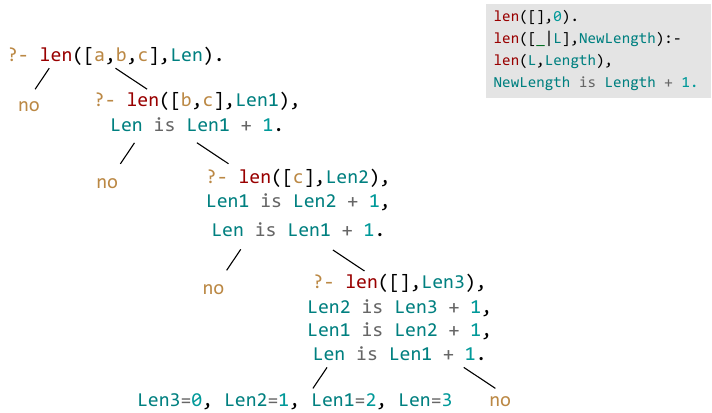
\includegraphics[width=0.5\linewidth]{images/parse_tree_acclen_2}
	\caption{Parse tree without tail recursion}
	\label{fig:parsetreeacclen2}
\end{figure}

\begin{figure}[h]
\centering
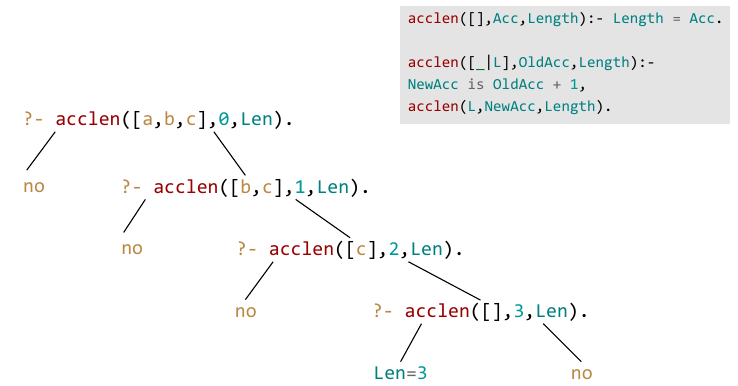
\includegraphics[width=0.5\linewidth]{images/parse_tree_acclen_tail_recursion}
\caption{Parse tree with tail recursion}
\label{fig:parsetreeacclentailrecursion}
\end{figure}

\paragraph{Example: Maximum of integer list \lstinline|max([1,2,3]).|}

%TODO: Notizen \mu

\subsection{Compiling Prolog Programs}

Prolog is based on a restricted subset of \emph{First order Predicate Calculus with Equality (FoPCe)}.

Horn Clauses is a clause with at most one un-negated (aka positive) literal. They have better computational properties.

\paragraph{Example} \hfill \\
\begin{figure}[H]
\centering
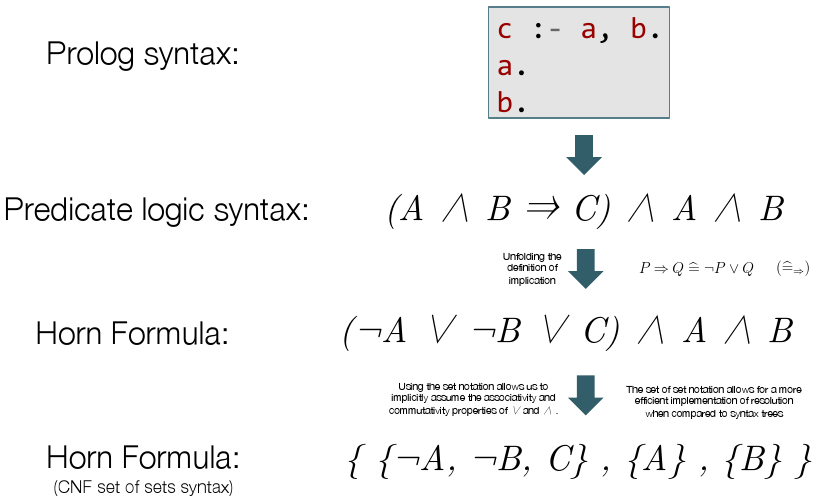
\includegraphics[width=0.4\linewidth]{images/prolog_to_horn_formula}
\caption{Prolog to Horn Formula transition}
\label{fig:prologtohornformula}
\end{figure}

A Horn Formula is a Horn Clause in CNF.

%TODO: Often used examples like, append, reverse, member(of), delete etc.

\section{Lambda calculus}

There are many variants of lambda calculus; but basically they all express computation based on function abstraction and application using variable binding and substitution. We currently only consider ''pure untyped'' lambda calculus.

Reserved words of this language are: ''$\lambda$'', ''.'' , ''('' and '')''. The ''='' and ''$\vdash$'' word are also reserved for predicates.

Haskell is based on Lambda Calculus.


\subsection{Sequent LC}
With LC, we also use the syntax $H \vdash G$. There are two language elements:

\begin{description}
	\item[Predicate $P$] $::= M=M$
	\item[$\lambda$-Terms $M$] $::= \underbrace{x}_{\mathllap{\text{Variable}}} | \overbrace{\lambda x. M}^{\mathclap{\lambda \text{ abstraction  (anonymous function)}}} | \underbrace{M M}_{\mathrlap{\text{Application of one } \lambda \text{ -term to another}}}$
\end{description}


\subsubsection{Binding Rules}
\begin{itemize}
	\item $\lambda x. M_1 M_2$ represents $\lambda x.(M_1 M_2)$ (Application binds tighter than abstraction)
	\item $M_1 M_2 M_3$ represents $(M_1 M_2) M_3$ (Application is left associative).
\end{itemize}

\subsubsection{Free and Bound Variables}

We have the same system of free and bound variables as in BasicPC:

\[
	(\lambda \underbrace{y.y}_{\mathclap{\text{bound}}}) \underbrace{a b}_{\mathclap{\text{free}}}
\]

\subsubsection{$\beta$-reduction rule}

LC contains only one proof rule schema of major significance: $\beta$-reduction.  This rule defines what function applications means in the context of the lambda calculus.

It means that we can prove $(\lambda y.y) 5$ is the same as $5$, because we replace the bound variable $y$ (literally the first letter after the $\lambda$) in the statement after the dot.

\begin{figure}[H] %TODO: Rewrite as real formula.
\centering
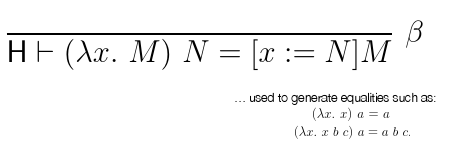
\includegraphics[width=0.5\linewidth]{images/beta_reduction}
\caption{Beta reduction rule}
\label{fig:betareduction}
\end{figure}


We can simply apply this proof with $\because$, for example:

\[
	\frac{(\lambda y.y) a b}{= a b} \because \beta
\]

\subsubsection{All LC rules}

\begin{figure}[H]
\centering
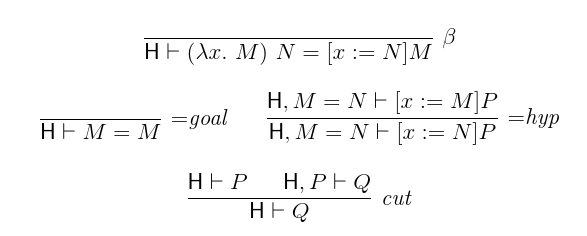
\includegraphics[width=0.7\linewidth]{images/lc_rules}
\caption{Overview lambda calculus rules}
\label{fig:lcrules}
\end{figure}


\subsection{Computation in LC}
Computation in lambda calculus is usually called ''reduction'': we make our statement easier.

\subsubsection{Halting problem}

We can represent endless loops in LC: $(\lambda x. x x) (\lambda x . x x)$. Therefore, the halting problem cannot be solved.

\subsubsection{Functions}

Functions in LC are first class citizens and can therefore be written like e.g. $\sin x$.

How are functions with multiple arguments possible? Using $M M$, we can create expressions, that are applied to multiple statements. We create \emph{higher order} functions with nested functions. The first function returns a function etcetera.




\section{Functional Programming (Haskell)}

\section{Multi-Paradigm Programming (Scala)}


\appendix

% Code Listings
\lstlistoflistings

% List of figures
\listoffigures

% List of tables
\listoftables

% Bibliography
\bibliographystyle{plain} 
\bibliography{literatur}

\end{document}
